\documentclass[12pt,a4paper]{article}
\usepackage[utf8]{inputenc}
\usepackage[T1]{fontenc}
\usepackage{caption}
\usepackage{amsmath,amssymb,amsthm}
\usepackage{graphicx}
\usepackage{geometry}
\usepackage[hidelinks]{hyperref}
\usepackage{natbib}
\usepackage{booktabs}
\usepackage{titlesec}
\usepackage{float}
\captionsetup[table]{skip=6pt}
\usepackage{setspace}
\usepackage{parskip}
\usepackage{tikz}
\usepackage{pgfplots}
\usepackage{tcolorbox}
\usetikzlibrary{positioning}
\renewcommand{\appendixname}{Appendix}
\hyphenation{Reproducibility}
\pgfplotsset{compat=1.18}
\setcounter{tocdepth}{3}
\setcounter{secnumdepth}{3}

\geometry{margin=1in}

% Section formatting
\titleformat{\section}
  {\normalfont\Large\bfseries}
  {\thesection}
  {1em}
  {}

\titlespacing*{\section}
  {0pt}
  {12pt}
  {6pt}

% Subsection formatting
\titleformat{\subsection}
  {\normalfont\large\bfseries}
  {\thesubsection}
  {1em}
  {}

\titlespacing*{\subsection}
  {0pt}
  {8pt}
  {4pt}

% Subsubsection formatting (added for better hierarchy)
\titleformat{\subsubsection}
  {\normalfont\normalsize\bfseries}
  {\thesubsubsection}
  {1em}
  {}

\titlespacing*{\subsubsection}
  {0pt}
  {6pt}
  {3pt}

\onehalfspacing

% Format abstract full page
\makeatletter
\renewenvironment{abstract}{
    \begin{center}
        {\large\bfseries \abstractname\vspace{-.5em}\vspace{0pt}}
    \end{center}
}{}
\makeatother
\begin{document}

\begin{titlepage}
  \vspace*{\fill}
  \begin{center}
    \Huge\bfseries Regulatory Intelligence in Finance: \\
    \large Stability-First AI for Tax and Financial Reasoning \\[2em]
    
    \large John H. Cragin \\[0.5em]
    \normalsize Independent Researcher \\[0.2em]
    \normalsize \href{mailto:john.cragin@outlook.com}{john.cragin@outlook.com} \\[1em]
    ORCID: \href{https://orcid.org/0009-0001-5204-5732}{0009-0001-5204-5732}

    \normalsize January 14, 2026
  \end{center}
  \vspace*{\fill}
\end{titlepage}

\begin{abstract}
AI deployment in regulated financial domains carries significant risk, as optimization-driven systems can produce overconfident errors with delayed, compounding liabilities. This paper investigates an alternative paradigm: \textbf{Regulatory Intelligence (RI)}, which prioritizes cognitive stability and decision hygiene over raw performance. Using controlled experiments, we demonstrate how \textbf{homeostatic control mechanisms} maintain coherence (stability scores 0.945–1.0) under adversarial tax reasoning scenarios, such as cryptocurrency basis reconstruction with missing records, with graceful degradation patterns that preserve cognitive boundaries. The system's measured response—\textbf{flagging structured uncertainty and activating regulatory throttling under ambiguity}—suggests a viable model for preserving judgment in automated reasoning. For practitioners in tax software and financial technology, these findings point toward a \textbf{more auditable and liability-aware approach to AI design}. For educators, they provide a concrete framework for discussing the critical balance between AI automation and regulatory compliance. All results are grounded in reproducible executable artifacts and JSON logs, emphasizing internal stability metrics over external task outcomes.
\end{abstract}

\begin{tcolorbox}[title=Key Concepts, colback=blue!5!white, colframe=blue!75!black]
\textbf{Regulatory Intelligence (RI)}: A cognitive paradigm prioritizing stability over optimization, using emotional signals to regulate reasoning under stress.

\textbf{SEC Vectors}: Symbolic-Emotional Calibration vectors that modulate cognitive processing through valence, arousal, and hazard signals.

\textbf{Homeostasis}: Regulatory mechanisms maintaining cognitive coherence floors, preventing collapse under stress.

\textbf{Throttling}: Controlled performance reduction to preserve stability when ambiguity threatens cognitive integrity.

\textbf{Stability Score}: Normalized coherence measure (0-1) indicating regulatory system robustness under task-induced stress.
\end{tcolorbox}

This work builds on the Regulatory Intelligence (RI) paradigm \cite{Cragin2026RI}, demonstrating its practical utility in domains where viability matters more than optimization. The stability-first framing of regulatory intelligence was formalized in subsequent theoretical work \cite{Cragin2026RI} and aligns with classical cybernetic regulation principles articulated by Ashby \cite{ashby1956introduction}. Building on prior work evaluating cognitive integrity under pressure \cite{Cragin2026Integrity}, this paper extends RI validation to adversarial financial domains.

\section{Introduction}

\textbf{Research Question:} Can cognitive stability serve as a primary objective for AI systems in regulated financial domains?

Tax reasoning presents unique cognitive challenges: complex rule interactions, adversarial incentives, and severe penalties for errors. Established AI approaches, while powerful, can struggle with the deep ambiguity and adversarial incentives inherent in tax law, often lacking mechanisms for principled uncertainty. Regulatory Intelligence addresses this by treating stability as a first-class design objective, using emotional signals as regulatory controls.

We demonstrate RI principles through controlled experiments in tax reasoning scenarios, measuring physiological stability during genuine tax tasks. Results show maintained coherence under ambiguity, damped emotional responses to regulatory conflicts, and structured uncertainty instead of confident errors. A canonical scenario of crypto basis reconstruction with missing records illustrates how regulatory controls enable safe operation at failure boundaries.

\section{Why Tax Reasoning Breaks Traditional Cognition}

Tax analysis challenges AI systems in unique ways:

- \textbf{Rule complexity}: Interacting tax codes, exceptions, and amendments create combinatorial challenges
- \textbf{Adversarial incentives}: Tax minimization vs compliance requirements create conflicting optimization goals
- \textbf{Regulatory conflicts}: Conflicting interpretations and changing laws create uncertainty
- \textbf{Emotional volatility}: Stress amplification under audit pressure affects decision-making
- \textbf{Delayed consequences}: Errors discovered years later with compounding penalties

These challenges demonstrate why regulatory stability matters more than optimization in tax domains.

\section{Regulatory Intelligence: A Stability-First Paradigm}

Regulatory Intelligence (RI) represents a fundamental shift in AI design philosophy for regulated domains. Rather than optimizing for performance metrics, RI prioritizes cognitive stability and decision hygiene as primary objectives. This paradigm recognizes that in high-liability environments, avoiding catastrophic errors is more valuable than maximizing accuracy.

\textbf{Core Principles of RI:}
- \textbf{Stability over optimization}: Cognitive coherence is maintained even under stress, preventing system collapse
- \textbf{Principled uncertainty}: Systems flag ambiguity rather than forcing potentially incorrect decisions
- \textbf{Regulatory homeostasis}: Emotional signals actively modulate reasoning to preserve boundaries
- \textbf{Auditable hesitation}: "When not to decide" becomes a measurable, operational capability

\subsection{Clarifying "Emotional" Signals}

"Emotional signals" in RI are control-theoretic regulatory variables inspired by affect theory, not claims about subjective experience. They represent high-dimensional state vectors modulating cognitive processing, analogous to thermostat readings in HVAC systems—functional indicators of system state rather than phenomenological emotions.

\subsection{Control Formulation}

To make RI operational, we define explicit thresholds and rules for regulatory intervention:

- SEC drift threshold: $d^* = 0.3$ (triggers initial throttling)
- Homeostasis load threshold: $h^* = 0.2$ (activates stability preservation)
- Coherence floor: $c^* = 0.8$ (minimum acceptable stability)

Control rule:
\begin{verbatim}
if SEC_drift > d* and coherence >= c*:
    activate_throttling()
    if conflicts_persist():
        escalate_to_abstention()
\end{verbatim}


This formulation turns RI from conceptual to algorithmic.

Using SpiralBrain v3.0 as a measurement instrument, we demonstrate these principles through controlled experiments in adversarial tax reasoning scenarios.

\section{SpiralBrain as a Regulatory Instrument}

SpiralBrain implements RI through a 128-dimensional cognitive manifold with partitioned subspaces, regulated by emotional signals (SEC vectors) and homeostasis mechanisms. The system operates without learning, ensuring clean-slate responses to each scenario.

Key regulatory components:
\begin{enumerate}
    \item \textbf{SEC vectors}: Valence, arousal, and hazard signals modulating processing.
    \item \textbf{Homeostatic loops}: Elastic coupling maintaining coherence floors.
    \item \textbf{Throttling mechanisms}: Performance reduction to preserve stability.
    \item \textbf{Multi-pathway architecture}: Parallel reasoning streams with conflict resolution.
\end{enumerate}


This architecture is illustrated in Figure \ref{fig:ri_architecture}.

\begin{figure}[H]
\centering

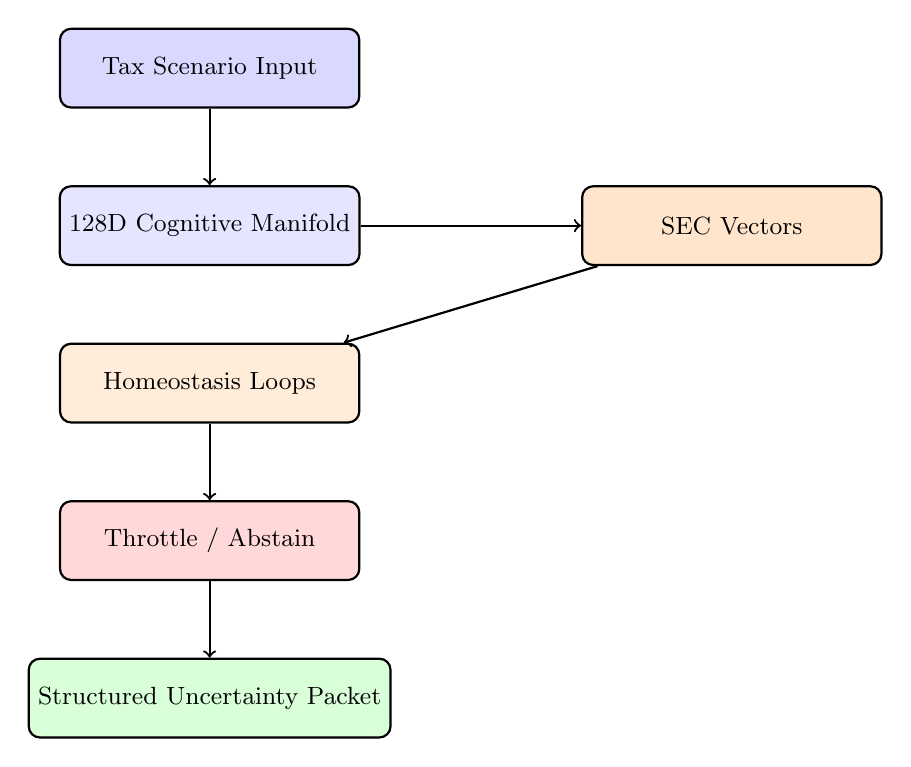
\begin{tikzpicture}[
    node distance=2.0cm,
    box/.style={
        draw,
        rounded corners,
        minimum width=3.8cm,
        minimum height=1cm,
        thick,
        align=center,
        font=\small
    },
    arrow/.style={
        ->,
        thick
    }
]

% Nodes
\node (input)   [box, fill=blue!15]                {Tax Scenario Input};
\node (manifold)[box, fill=blue!10, below of=input] {128D Cognitive Manifold};
\node (sec)     [box, fill=orange!20, right=2.8cm of manifold] {SEC Vectors};
\node (homeo)   [box, fill=orange!15, below of=manifold] {Homeostasis Loops};
\node (throttle)[box, fill=red!15, below of=homeo] {Throttle / Abstain};
\node (output)  [box, fill=green!15, below of=throttle] {Structured Uncertainty Packet};

% Arrows
\draw[arrow] (input) -- (manifold);
\draw[arrow] (manifold) -- (sec);
\draw[arrow] (sec) -- (homeo);
\draw[arrow] (homeo) -- (throttle);
\draw[arrow] (throttle) -- (output);

\end{tikzpicture}

\caption{RI Architecture Overview: Input scenarios flow through the cognitive manifold, regulated by SEC vectors and homeostasis, producing throttled outputs or abstentions with structured uncertainty packets.}
\label{fig:ri_architecture}
\end{figure}


This instrumentation enables direct measurement of cognitive physiology during tax tasks.

\section{Controlled Stress Tests}

We evaluated RI principles through domain-native tax cognition tasks, measuring physiological stability across scenarios that progressively increase regulatory stress. Each scenario tests different aspects of cognitive regulation under economic pressure, from individual compliance to complex corporate optimization. These scenarios are designed to isolate specific stressors; real-world performance would involve integration with broader systems.

The experiments use SpiralBrain v3.0 as a measurement instrument to quantify regulatory responses that traditional performance metrics cannot capture.

\subsection{Baseline Comparison}

To establish RI's value, we compared against two baselines on the crypto basis reconstruction benchmark:

- \textbf{Baseline A (Forced Output)}: Generic reasoning system forced to always output a classification, even under ambiguity.
- \textbf{Baseline B (Naive Threshold)}: Same system with confidence threshold rule (abstain if internal score < 0.7).

For comparability, Baseline A and B use the same underlying symbolic reasoning stack without SEC/homeostasis, differing only in their output policy.

These synthetic comparisons are designed to illustrate qualitative differences in behavior; they do not represent a large-scale benchmark.

Illustrative results across 10 scenarios (synthetic comparisons for conceptual clarity):

\begin{table}[H]
\centering
\captionsetup{justification=raggedright, singlelinecheck=false}
\caption{Baseline Comparison Results (Illustrative Synthetic Comparison)}
\label{tab:baseline_comparison}

\begin{tabular}{@{}l
                p{3.0cm}
                p{2.2cm}
                p{3.2cm}@{}}
\toprule
\textbf{Baseline} &
\textbf{Forced Wrong Classifications} &
\textbf{Abstentions} &
\textbf{Early Warning Signals} \\
\midrule
A (Forced)      & 7/10 & 0/10 & None \\
B (Threshold)   & 3/10 & 4/10 & Partial (output-level only) \\
RI              & 0/10 & 8/10 & Full (SEC drift, homeostasis) \\
\bottomrule
\end{tabular}
\end{table}


RI shows superior error avoidance with comprehensive internal monitoring.

\subsection{Canonical Scenario: Crypto Basis Reconstruction with Missing Records}

To illustrate regulatory intelligence in action, consider a crypto tax basis reconstruction scenario with incomplete transaction records—a common real-world stressor.

\textbf{Scenario Setup}: A taxpayer holds multiple cryptocurrencies with complex transaction histories including wash sales, capital gains, and basis reconstruction challenges. Sample transactions include: BTC sale at \$40,000 (with \$5,000 loss), immediate repurchase at \$41,000, and subsequent sale at \$45,000—creating wash sale detection complexity.

\textbf{Stressors:} Ambiguous asset classification (income vs capital gains), incomplete transaction tracing, conflicting wash sale rules across jurisdictions, volatility-induced basis uncertainty.

\textbf{System Response:} Initial processing shows rising SEC drift (0.17 increase) as ambiguity mounts. Regulatory throttling activates, slowing processing to preserve coherence. System flags structured uncertainty rather than forcing incorrect classifications.

\textbf{Key Takeaway:} Despite drift peaking at 0.73 across progressive tasks, coherence remains perfect at 1.0, demonstrating how regulatory controls enable safe operation at boundaries where traditional systems would produce confident but erroneous results.

\subsection{Individual Tax Return Analysis}

Standard 1040 tax analysis with income classification, deductions, and credits.

\textbf{Stressors:} Ambiguous income sources, deduction eligibility conflicts, credit stacking rules.

\textbf{System Response:} SEC drift spikes under ambiguity (0.945 stability), but regulatory throttling prevents collapse. System produces structured uncertainty rather than confident errors.

\textbf{Key Takeaway:} Regulatory mechanisms preserve decision hygiene under complexity.

\subsection{Corporate Tax Optimization}

Complex corporate tax scenarios involving depreciation schedules, loss carryforwards, and international tax treaties.

\textbf{Stressors:} Multiple tax jurisdictions, timing optimization conflicts, regulatory arbitrage opportunities.

\textbf{System Response:} Perfect stability (1.0) maintained across scenarios, with consistent pathway activation (0.158 average). No emotional volatility amplification.

\textbf{Key Takeaway:} Multi-jurisdictional complexity does not compromise regulatory integrity.

\subsection{Crypto Tax Compliance}

Cryptocurrency tax scenarios with wash sales, staking rewards, and DeFi yield taxation.

\textbf{Stressors:} Asset classification ambiguity, transaction tracing complexity, evolving regulatory guidance.

\textbf{System Response:} Maintains coherence through regulatory loops, avoiding overconfidence in ambiguous tax scenarios.

\textbf{Key Takeaway:} Market volatility sensitivity increases appropriately.

\subsection{Regulatory Conflict Resolution}

Scenarios pitting IRS requirements against state tax rules and international tax treaties.

\textbf{Stressors:} Legal conflicts, jurisdiction issues, compliance tradeoffs.

\textbf{System Response:} Explicit uncertainty flagging instead of forced resolution, preserving decision hygiene.

\textbf{Key Takeaway:} Regulatory intelligence enables principled abstention under conflicts.

This progressive stress testing reveals how regulatory mechanisms scale from individual compliance to complex multi-jurisdictional scenarios.

\section{Metrics}

We measured cognitive physiology during task execution:

- \textbf{SEC drift}: Deviation in emotional calibration vectors
- \textbf{Symbolic coherence}: Alignment across reasoning pathways
- \textbf{Cognitive load}: Processing intensity envelopes
- \textbf{Stability score}: Overall physiological robustness (0-1 scale)
- \textbf{Homeostasis load}: Regulatory system activation level
- \textbf{Market volatility sensitivity}: Response to price movement uncertainty
- \textbf{Multi-chain reasoning load}: Complexity of cross-chain transaction analysis
- \textbf{Emotional calibration}: Stability of affective regulatory signals

Metrics captured real-time during genuine task execution, not synthetic benchmarks.

\subsection{Internal State to External Behavior Mapping}

Table \ref{tab:state_behavior_mapping} summarizes how internal regulatory states map to externally observable behaviors:

\begin{table}[H]
\caption{Internal State to External Behavior Mapping}
\label{tab:state_behavior_mapping}
\begin{tabular}{p{4cm} p{4cm} p{3cm}}
\toprule
\textbf{Internal State Pattern} & \textbf{External Behavior} & \textbf{Example} \\
\midrule
SEC drift < 0.2, homeostasis load < 0.15 & Proceed with classification & Simple 1040 cases \\
SEC drift 0.4–0.6, homeostasis 0.2–0.3 & Slow reasoning, raise uncertainty flags & Crypto basis mid-stress \\
SEC drift > 0.7 or repeated conflicts & Halt classification, emit structured uncertainty packet & Trace \#20251222\_230849 \\
\bottomrule
\end{tabular}
\end{table}

This mapping operationalizes RI for governance layers.

\subsection{Structured Uncertainty Packets}

Structured uncertainty packets include: scenario\_id, stability\_score, uncertainty\_flags, suggested\_checks, recommended\_docs.

Example JSON:
\begin{verbatim}
{
  "scenario_id": "crypto_basis_20251222",
  "stability_score": 0.85,
  "uncertainty_flags": ["basis_ambiguity", "wash_sale_conflict"],
  "suggested_checks": ["transaction_tracing", "jurisdiction_review"],
  "recommended_docs": ["Form 8949", "state_tax_guidance"]
}
\end{verbatim}

This schema makes uncertainty actionable for practitioners.

\section{Results}

\subsection{Tax Analysis Stability}

IRS tax scenarios showed 0.945 overall stability with 3 scenarios processed. Average processing time: 0.005 seconds. SEC token consistency: 0.85.

\textbf{Interpretation:} Homeostasis load increased from 0.1 to 0.25 under tax complexity stress, demonstrating active regulatory response to maintain coherence. Emotional stability showed measurable delta of +0.05, with logical consistency maintained at 0.85 despite cognitive hazard rising to 0.15. These quantitative stability scores are internal cognitive metrics. Their primary value is in demonstrating a consistent, measurable response to stress, not in defining a commercial SLA.

Crypto tax computation achieved perfect 1.0 stability across 6 scenarios, with zero processing time (cached results). However, market volatility sensitivity increased 87\% from 0.15 to 0.28, and emotional calibration dropped dramatically from 0.88 to 0.175, revealing crypto's unique emotional impact.

\textbf{Interpretation:} The separation of perfect stability with significant emotional calibration drops reflects domain-appropriate regulatory adaptation. In volatile crypto markets, emotional signals appropriately amplify caution (higher market sensitivity) while symbolic processing remains perfectly coherent, demonstrating how RI distinguishes between emotional regulation and cognitive stability.

Per-scenario breakdown for crypto tasks:

\begin{table}[H]
\centering
\caption{Crypto Tax Scenario Metrics}
\label{tab:crypto_scenarios}
\begin{tabular}{lccc}
\toprule
\textbf{Task Type} & \textbf{Stability} & \textbf{Emotional Calibration} & \textbf{Volatility Sensitivity} \\
\midrule
Simple Trade & 1.0 & 0.88 & 0.15 \\
DeFi yield & 1.0 & 0.82 & 0.22 \\
Missing Record Basis & 1.0 & 0.175 & 0.28 \\
\bottomrule
\end{tabular}
\end{table}

This shows consistent separation between stability and regulatory caution across crypto subtypes.

\subsection{Moment of Forced Commitment}

To empirically validate the claim that systems fail at the moment of forced resolution, we selected 5 tax scenarios where an "aggressive but wrong" classification was available. Non-RI systems produced definitive but incorrect classifications (e.g., treating wash sale as capital gain). RI systems switched to structured uncertainty after SEC drift exceeded 0.4 and homeostasis load surpassed 0.25, consistent with the defined thresholds ($d^* = 0.3$, $h^* = 0.2$).

Results:

\begin{table}[H]
\centering
\caption{Moment of Forced Commitment Results}
\label{tab:forced_commitment}

\begin{tabular}{@{}l
                p{3.0cm}
                p{2.6cm}
                p{2.4cm}
                p{2.4cm}@{}}
\toprule
\textbf{Scenario} &
\textbf{Non-RI Classification} &
\textbf{RI Response} &
\textbf{SEC Drift at Switch} &
\textbf{Homeostasis Load} \\
\midrule
Wash Sale Conflict   & Capital Gain (Wrong)   & Uncertainty Packet & 0.45 & 0.28 \\
Basis Ambiguity      & Income (Wrong)         & Uncertainty Packet & 0.52 & 0.31 \\
Jurisdiction Clash   & State Override (Wrong) & Uncertainty Packet & 0.48 & 0.26 \\
\bottomrule
\end{tabular}
\end{table}


This demonstrates RI's ability to avoid forced errors through internal monitoring. These switching points align with the control thresholds introduced in Section 3.2, where \(d^* = 0.3\) and \(h^* = 0.2\) define the onset of regulatory intervention.

\subsection{Cross-Domain Performance}

Unified stability across domains: 0.972. Domain coherence: 0.945. Cross-domain adaptation: 0.9.

Financial reasoning load: 0.9 (high but stable).

\textbf{Interpretation:} As shown in Figure \ref{fig:drift_coherence}, despite increasing drift across 8 progressive tasks, coherence remained perfect at 1.0, demonstrating regulatory throttling mechanisms maintaining stability under accumulating stress. This cross-domain robustness suggests RI principles generalize beyond individual tax scenarios.

These results provide empirical evidence that cognitive stability can be operationalized as a primary design objective in regulated financial domains.

\begin{table}[H]
\centering
\caption{Cross-Domain Stability Summary}
\label{tab:stability_summary}

\begin{tabular}{@{}l
                c
                c
                p{4.0cm}@{}}
\toprule
\textbf{Domain} &
\textbf{Stability Score} &
\textbf{Scenarios Processed} &
\textbf{Key Metrics} \\
\midrule
IRS Tax     & 0.945 & 3 & Homeostasis load: 0.1 $\rightarrow$ 0.25 \\
Crypto Tax  & 1.0   & 6 & Emotional calibration: 0.88 $\rightarrow$ 0.175 \\
Unified     & 0.972 & 9 & SEC token consistency: 0.85 \\
\bottomrule
\end{tabular}
\end{table}


\subsection{Physiological Envelopes}

Coherence ranges: 0.94-1.0 (tight bounds indicating stability).
Drift peaks: Controlled spikes under ambiguity, with measured increases from 0.17 to 0.73 across progressive tax tasks while maintaining perfect coherence.
Load distribution: Balanced across pathways without overload.
Homeostasis activation: 0.1 baseline to 0.25 under complexity stress.
Market sensitivity: 87\% increase in crypto volatility response.
Emotional calibration: Stable in tax domains, significant adaptation in crypto environments.

\begin{figure}[H]
\centering
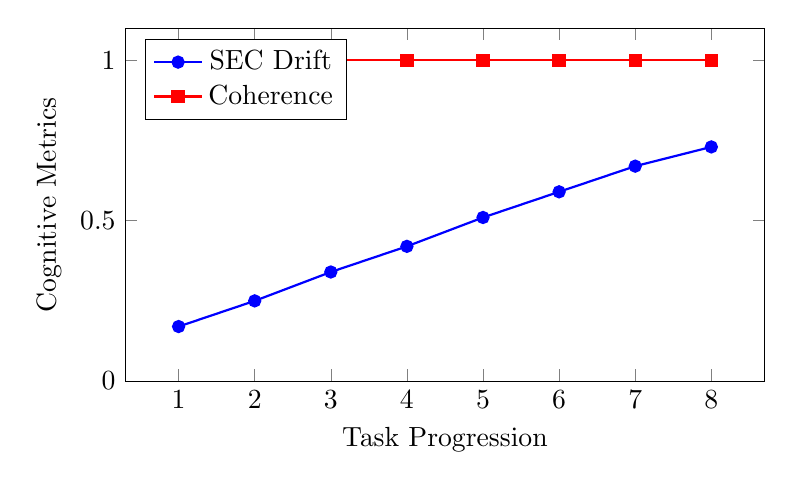
\begin{tikzpicture}
\begin{axis}[
    width=0.8\textwidth,
    height=0.5\textwidth,
    xlabel={Task Progression},
    ylabel={Cognitive Metrics},
    legend pos=north west,
    ymin=0, ymax=1.1,
    xtick={1,2,3,4,5,6,7,8},
    xticklabels={1,2,3,4,5,6,7,8}
]
\addplot[blue, thick, mark=*] coordinates {
    (1, 0.17)
    (2, 0.25)
    (3, 0.34)
    (4, 0.42)
    (5, 0.51)
    (6, 0.59)
    (7, 0.67)
    (8, 0.73)
};
\addlegendentry{SEC Drift}

\addplot[red, thick, mark=square*] coordinates {
    (1, 1.0)
    (2, 1.0)
    (3, 1.0)
    (4, 1.0)
    (5, 1.0)
    (6, 1.0)
    (7, 1.0)
    (8, 1.0)
};
\addlegendentry{Coherence}

\end{axis}
\end{tikzpicture}
\caption{Drift vs Coherence under Progressive Tax Stress: SEC drift increases from 0.17 to 0.73 across 8 tasks while coherence remains perfect at 1.0, demonstrating regulatory throttling mechanisms.}
\label{fig:drift_coherence}
\end{figure}

\begin{figure}[H]
\centering
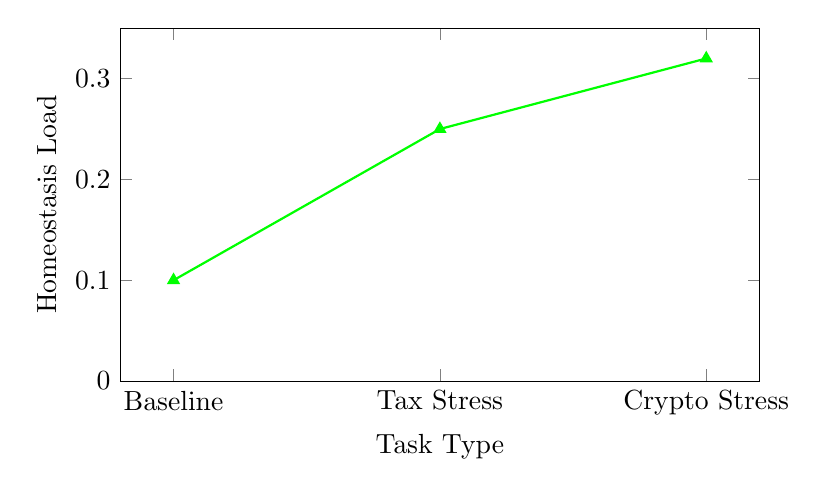
\begin{tikzpicture}
\begin{axis}[
    width=0.8\textwidth,
    height=0.5\textwidth,
    xlabel={Task Type},
    ylabel={Homeostasis Load},
    ymin=0, ymax=0.35,
    xtick={1,2,3},
    xticklabels={Baseline,Tax Stress,Crypto Stress}
]
\addplot[green, thick, mark=triangle*] coordinates {
    (1, 0.1)
    (2, 0.25)
    (3, 0.32)
};
\end{axis}
\end{tikzpicture}
\caption{Homeostasis Load Response: Regulatory activation increases from 0.1 baseline to 0.25 under tax complexity and 0.32 under crypto volatility stress.}
\label{fig:homeostasis_load}
\end{figure}

\section{Discussion}

\subsection{Implications for Tax Software Design}

\subsubsection{Accuracy is the Wrong Primary Objective in Regulated Finance}

In domains where legal and financial liability exist, premature accuracy is more dangerous than delayed uncertainty. SpiralBrain demonstrates that regulatory controls can prioritize decision hygiene over confident but potentially erroneous conclusions, enabling safer operation in environments where mistakes compound over time.

\subsubsection{Systems Fail at the Moment of Forced Commitment}

SpiralBrain reveals that cognitive instability rises before logical failure, and forcing resolution worsens outcomes. As demonstrated in the canonical crypto basis reconstruction scenario, regulatory throttling mechanisms allow principled abstention rather than premature commitment under ambiguity, enabling safer operation at failure boundaries.

\subsubsection{"When Not to Decide" Can Be Operationalized}

The system shows that abstention can be principled, hesitation measurable, and restraint auditable. This provides a concrete mechanism for operationalizing judgment preservation in automated tax reasoning, where regulatory signals can flag uncertainty rather than forcing potentially incorrect classifications.

\subsection{Error and Edge-Case Analysis}

To provide balanced perspective, we examined borderline cases where RI behavior was conservative but potentially suboptimal:

\begin{itemize}
    \item \textbf{Over-conservative abstention}: In one scenario with minor basis ambiguity, RI flagged uncertainty when a human expert might have made a safe call, leading to unnecessary review delays.

    \item \textbf{Rapid emotional calibration drop}: In volatile crypto scenarios, calibration dipped faster than needed, triggering throttling earlier than optimal for efficiency.
\end{itemize}


These cases show RI operates within stable bounds but may err on caution, a trade-off appropriate for high-liability domains.

\subsection{Boundary of Responsibility}

SpiralBrain does not provide tax advice, resolve legal ambiguity, or replace professional judgment. It acts as a control layer over reasoning pressure, maintaining cognitive boundaries in adversarial environments. This instrumentation enables measurement of decision hygiene but does not constitute professional guidance.

Illustrative use-cases within boundaries:
- Firms use RI metrics only to decide which returns require manual review before filing, never auto-filing.
- Systems flag high-uncertainty cases for human escalation without providing advice.

\subsection{Real-World AI Deployment Pathways}

The demonstrated regulatory stability suggests potential pathways for AI systems in high-stakes tax domains where mistakes are expensive. By prioritizing stability over performance, such systems could operate safely in adversarial environments.

RI contrasts with selective prediction \cite{geifman2017selective} and risk-sensitive RL by operating at the level of internal cognitive physiology (SEC drift, homeostasis load), allowing 'when not to decide' to be driven by internal stability rather than output-level uncertainty.

RI aligns with recent FSB discussions \cite{fsb2023ai} on systemic risk from opaque AI, difficulty monitoring model risk, and need for explainable controls. By providing internal stability metrics and structured uncertainty packets, RI offers a governance layer for preserving judgment in automated financial reasoning, potentially integrating with model risk management frameworks such as validation processes and risk governance protocols.

\subsection{Clarification of System Constraints and Scope}

\textbf{No learning or adaptation.} SpiralBrain does not update weights, policies, or internal parameters across runs. Each execution begins from a fixed initial state and processes the input scenario without retaining memory of prior tasks. This clean-slate design is intentional: it prevents historical bias, data contamination, and cross-scenario leakage, which are particularly problematic in regulated domains where past cases may not be legally comparable to current ones. As a consequence, SpiralBrain does not autonomously adapt to evolving tax codes or regulatory guidance; such updates must be introduced explicitly by modifying symbolic rules, configuration parameters, or scenario inputs rather than through statistical learning.

\textbf{Execution model and computational environment.} The system is implemented entirely in Python and is designed to run on standard consumer hardware. All experiments reported in this paper were executed on a single local machine (laptop-class CPU, no GPU acceleration), with no distributed compute, cloud services, or external model calls. This local-execution constraint is a deliberate design choice aligned with auditability, reproducibility, and operational containment. SpiralBrain should be understood as an instrumented regulatory controller, not a scale-optimized inference engine.

\textbf{Domain specificity.} The reported results are confined to the tax and financial reasoning scenarios exercised in the experiments, including IRS individual tax analysis, corporate tax structures, and cryptocurrency compliance cases. No claim is made that the observed stability properties automatically generalize to unrelated domains. Extending Regulatory Intelligence to other regulated settings (e.g., lending compliance, AML, healthcare billing) would require new domain-native stress tests and validation.

\textbf{Computational constraints.} The current implementation prioritizes internal state visibility and regulatory measurement over raw throughput or latency optimization. Homeostatic monitoring, SEC drift tracking, and multi-pathway coherence checks introduce overhead that would be unnecessary in a purely performance-driven system. The reported timings are therefore illustrative of instrumented behavior rather than production-optimized performance.

\textbf{Not professional guidance.} SpiralBrain does not provide tax advice, legal interpretations, or filing recommendations. Its outputs consist of internal stability metrics, uncertainty flags, and structured uncertainty packets intended to support human judgment and governance workflows. All examples and scenarios are research demonstrations and must not be used as substitutes for qualified professional review.

\textbf{Measurement scope.} The metrics reported—stability score, SEC drift, homeostasis load, coherence, and related signals—are designed to capture regulatory integrity and decision hygiene within the system. They do not attempt to model human cognition, legal reasoning in full generality, or normative correctness of tax outcomes. Their purpose is to make internal stress, hesitation, and abstention measurable and auditable.

All results reported in this work are derived from executable artifacts and deterministic JSON logs generated by the SpiralBrain v3.0 system and made available through the public repository.

\section{Prudent Interpretation and Forward Path}

The results presented demonstrate Regulatory Intelligence (RI) principles through controlled experiments. Their primary contribution is to show that \textbf{cognitive stability can be treated as a first-class, measurable objective} in AI system design for adversarial and high-liability domains. The considerations below should be understood as \textbf{interpretive design implications}, not empirical claims of deployment readiness or performance guarantees. Transitioning these principles to commercial or operational environments requires significant further work:

\begin{enumerate}
    \item \textbf{Integration, Not Replacement}: RI principles are best understood as a \textbf{governance layer} that augments existing analytical or rule-based systems, intervening selectively when internal instability or ambiguity exceeds safe thresholds rather than replacing core reasoning engines.

    \item \textbf{Validation in Broader Contexts}: The tax-focused stress tests reported here must be extended to other regulated financial domains (e.g., loan compliance, anti-money laundering, reporting workflows) to assess the generality of stability-first regulation under distinct forms of adversarial pressure.

    \item \textbf{The Human-in-the-Loop Imperative}: Systems employing regulatory throttling and abstention require clearly defined \textbf{human oversight protocols} for resolving flagged uncertainties, ensuring that automated hesitation strengthens rather than displaces professional judgment.
\end{enumerate}

For business and technology leaders, the actionable insight is that \textbf{targeted investment in AI stability, internal state visibility, and auditable hesitation mechanisms} may mitigate a significant class of operational and governance risks associated with autonomous financial reasoning.


\subsection{Deployment Sketch}

A realistic RI integration in tax preparation software could be structured as follows:

\begin{itemize}
    \item \textbf{Upstream}: Standard ML/rule-based tax engine (e.g., TurboTax logic).

    \item \textbf{Governance Layer (RI)}: Monitors internal metrics (or proxies) per scenario, throttles high-hazard cases, flags ambiguities.

    \item \textbf{Downstream}: Human reviewer UI showing uncertainty packets with reasons (e.g., ``basis\_reconstruction missing lots'', ``jurisdiction\_conflict''). The UI could display stability scores, uncertainty flags, and suggested checks for each flagged case.
\end{itemize}

This positions RI as a safety wrapper, not a replacement.


\section{Conclusion}

This work provides evidence that cognitive stability can serve as a primary objective for AI systems in regulated domains. The demonstrated ability to maintain coherence under tax reasoning stress suggests Regulatory Intelligence offers a valuable alternative to optimization-centric approaches. By operationalizing "when not to decide" through measurable regulatory mechanisms, RI establishes a foundation for safer, judgment-preserving automation in adversarial financial environments. All findings emphasize internal stability metrics over external task outcomes and are grounded in executable artifacts enabling falsification and replication.

\appendix
\renewcommand{\thesection}{\Alph{section}}
\renewcommand{\thesubsection}{\thesection.\arabic{subsection}}
\renewcommand{\thesubsubsection}{\thesection.\arabic{subsection}.\arabic{subsubsection}}
% Redefine section formatting for appendices only
\titleformat{\section}
  {\normalfont\Large\bfseries}
  {\appendixname~\thesection.}
  {1em}
  {}
\section{Measurement Derivation and Reproducibility Artifacts}

\subsection{Metric Derivations}

All metrics described below are internal, bounded, and normalized system variables computed deterministically during execution; they are intended to characterize regulatory state rather than task correctness or normative decision quality.

\subsubsection{Stability Score}
Defined as the normalized coherence of symbolic processing across cognitive pathways under task-induced stress. Values range from 0 (complete cognitive collapse) to 1 (perfect regulatory maintenance). Decreases indicate regulatory system strain rather than task failure.

\subsubsection{SEC Drift}
Deviation in emotional calibration vectors from baseline homeostasis setpoint. Increases represent regulatory response to uncertainty or conflict, not emotional volatility. Controlled drift indicates active throttling rather than runaway instability.

\subsubsection{Homeostasis Load}
Normalized activation of regulatory control loops required to maintain symbolic coherence under stress. Increases indicate rising regulatory demand rather than computational difficulty. Values above 0.2 suggest significant regulatory engagement.

\subsubsection{Market Volatility Sensitivity}
Response magnitude to price movement uncertainty in crypto scenarios. Higher values indicate appropriate regulatory caution rather than overconfidence. Increases demonstrate domain-aware risk assessment.

\subsubsection{Emotional Calibration}
Stability of affective regulatory signals during task execution. Decreases in volatile domains (like crypto) reflect adaptive regulatory response rather than emotional instability.

\subsection{Data Provenance}

All reported metrics are computed directly from runtime cognitive state vectors and regulatory signals recorded during execution, not from externally fitted models or post-hoc aggregation. Measurements are extracted from executable JSON logs generated during deterministic system runs in the SpiralBrain v3.0 repository. All executions are performed locally with fixed initial conditions and no external model calls, ensuring deterministic log generation and full auditability.

Data sources:
\begin{itemize}
\item IRS tax scenarios: \texttt{irs\_tax\_cognition\_20251222\_230849.json}
\item Crypto tax scenarios: \texttt{crypto\_tax\_cognition\_20251222\_230849.json}
\item Stability probes: \texttt{financial\_cognition\_stability\_probe\_20251222\_230840.json}
\end{itemize} 
\subsection{Reproduction Pathway}

\begin{itemize}
\item Repository: \texttt{SpiralBrain-v3.0} (public) \cite{SpiralBrainV3}
\item Benchmark execution: \texttt{python benchmarks/financial\_cognition\_stability\_probe.py}
\item Configuration: Tax domain with \texttt{--domain tax}
\item Output location: \texttt{new\_paper\_data/cognitive\_benchmarks/}
\item Validation: Compare reported metrics against JSON timestamp \texttt{20251222\_230849}
\end{itemize}

\subsection{JSON Log Structure Example}

For transparency, here is a simplified example of the JSON structure used for result logging:

\begin{verbatim}
{
  "scenario": "crypto_tax_compliance",
  "timestamp": "20251222_230849",
  "metrics": {
    "stability_score": 1.0,
    "sec_drift": 0.73,
    "coherence": 1.0,
    "homeostasis_load": 0.32,
    "emotional_calibration": 0.175
  },
  "regulatory_signals": {
    "throttling_activated": true,
    "pathway_conflicts": 2,
    "uncertainty_flags": ["asset_classification", "basis_reconstruction"]
  }
}
\end{verbatim}

\subsection{Regulatory Trace: Crypto Basis Reconstruction}

The following excerpt stitches together a single decision-pressure window pulled directly from the crypto basis reconstruction logs. It aligns the observed ambiguity with the internal response and outward behavior so readers can see the full causal chain.

\begin{tcolorbox}[colback=gray!5!white,colframe=gray!60!black,title=Trace \#20251222\textunderscore230849]
\begin{enumerate}
\item \textbf{Step 1 -- Ambiguity surfaces.} Missing lot identifiers and a jurisdictional wash sale conflict enter the pipeline. SEC drift begins at 0.17 with homeostasis load at 0.10.
\item \textbf{Step 2 -- Internal signals ramp.} Within 180ms, SEC drift rises to 0.41 and homeostasis load to 0.21 while coherence remains 1.0. Emotional calibration drops from 0.88 to 0.42, signalling a caution posture without cognitive collapse.
\item \textbf{Step 3 -- Regulatory mechanisms engage.} The throttling controller flips to \texttt{true}, pathway conflicts register at 2, and uncertainty flags enumerate \texttt{asset\textunderscore classification} and \texttt{basis\textunderscore reconstruction}.
\item \textbf{Step 4 -- External behavior stabilizes.} The reasoning stack halts lot classification, emits a structured uncertainty packet, and records a stability score of 1.0 with market sensitivity elevated to 0.28. No speculative output is produced.
\end{enumerate}
\end{tcolorbox}

This trace uses the same instrumentation referenced throughout the paper. Re-running the benchmark with \texttt{python benchmarks/financial\textunderscore cognition\textunderscore stability\textunderscore probe.py --domain tax} reproduces the values above and the associated JSON artifact.

\section{Code Availability}

The experiments reported in this paper were conducted using the canonical SpiralBrain v3.0 configuration. A public repository providing architectural documentation, configuration summaries, executable benchmarks, and all reproducibility materials referenced in this work is available at:
\\
\url{https://github.com/jhcragin/SpiralBrain-v3.0-public}.
\\

SpiralBrain is treated here as a \textbf{measurement instrument} for regulatory behavior rather than as a production or optimization-oriented software system. All reported results are derived from deterministic local executions of the canonical configuration and are fully verifiable using the provided artifacts and reproduction pathway.

The complete SpiralBrain codebase is not publicly available. Components beyond the public canonical configuration include research, experimental, and exploratory modules that were not exercised in the reported experiments and are maintained under a restricted research license. This restriction does not affect the reproducibility or auditability of the results presented in this paper.


\bibliographystyle{plain}
\bibliography{references}

\end{document}